% Plane Sections of the Cylinder - Dandelin Spheres
% Author: Hugues Vermeiren
\documentclass[border=3pt]{standalone}
\usepackage{tikz, tikz-3dplot}
\tikzset{
	MyPersp/.style={scale=1.8,x={(-0.8cm,-0.3cm)},y={(0.8cm,-0.3cm)},
    z={(0cm,1cm)}},
    coord/.style={x={(1cm,0cm)}, y={(0cm,1cm)}, z={(-0.4cm,-0.0cm)}},
 % MyPersp/.style={scale=1.5,x={(0cm,0cm)},y={(1cm,0cm)},
   % z={(0cm,1cm)}}, % uncomment the two lines to get a lateral view
	MyPoints/.style={fill=white,draw=black,thick}
		}
\usetikzlibrary{3d}
 \tikzset{zxplane/.style={canvas is zx plane at y=#1}}
 \tikzset{yxplane/.style={canvas is yx plane at z=#1}}
 \tikzset{zyplane/.style={canvas is zy plane at x=#1}}

\def\centerarc[#1](#2)(#3:#4:#5)% Syntax: [draw options] (center) (initial angle:final angle:radius)
    { \draw[#1] ($(#2)+({#5*cos(#3)},{#5*sin(#3)})$) arc (#3:#4:#5); }
\begin{document}

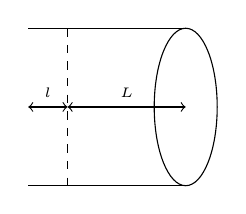
\begin{tikzpicture}[coord,font=\large]

  % \begin{scope}[zxplane=0]
  %    \draw (0,0) circle (1cm);
  %    \draw (-1,0) -- (1,0) (0,-1) -- (0,1);
  %  \end{scope}

   \begin{scope}[zyplane=0]
     % \draw (0,0) circle (1cm);
     % \draw (0,0) arc (20:270:1cm);
     \centerarc[dashed](0,0)(90:270:1);
     \centerarc[](0,0)(270:450:1);
     % \draw (-1,0) -- (1,0) (0,-1) -- (0,1);
   \end{scope}

   \draw (0,1,0) -- (2,1,0);
   \draw (0,-1,0) -- (2,-1,0);

   \draw[<->, thin] (0.5,0,0) -- node[above] {\tiny $L$} (2,0,0);
   \draw[<->, thin] (0,0,0) --  node[above] {\tiny $l$}(0.5,0,0);

    \draw[dashed, very thin] (0.5,1,0) -- (0.5,-1,0);

    \begin{scope}[zyplane=2]
     \draw (0,0) circle (1cm);
     % \draw (-1,0) -- (1,0) (0,-1) -- (0,1);
   \end{scope}

   % \begin{scope}[zyplane=0]
   %   \draw (0,0) circle (1cm);
   %   \draw (-1,0) -- (1,0) (0,-1) -- (0,1);
   % \end{scope}

	% the base circle is the unit circle in plane Oxy
	\def\h{2.5}% Heigth of the ellipse center (on the axis of the cylinder)
	\def\a{35}% angle of the section plane with the horizontal
	\def\aa{35}% angle that defines position of generatrix PA--PB
	\pgfmathparse{\h/tan(\a)}
  \let\b\pgfmathresult
	\pgfmathparse{sqrt(1/cos(\a)/cos(\a)-1)}
  \let\c\pgfmathresult %Center Focus distance of the section ellipse.
	\pgfmathparse{\c/sin(\a)}
  \let\p\pgfmathresult % Position of Dandelin spheres centers
                       % on the Oz axis (\h +/- \p)
	% \coordinate (A) at (2,\b,0);
	% \coordinate (B) at (-2,\b,0);
	% \coordinate (C) at (-2,-1.5,{(1.5+\b)*tan(\a)});
	% \coordinate (D) at (2,-1.5,{(1.5+\b)*tan(\a)});
	% \coordinate (E) at (2,-1.5,0);
	% \coordinate (F) at (-2,-1.5,0);
	% \coordinate (CLS) at (0,0,{\h-\p});
	% \coordinate (CUS) at (0,0,{\h+\p});
	% \coordinate (FA) at (0,{\c*cos(\a)},{-\c*sin(\a)+\h});% Focii
	% \coordinate (FB) at (0,{-\c*cos(\a)},{\c*sin(\a)+\h});
	% \coordinate (SA) at (0,1,{-tan(\a)+\h}); % Vertices of the
 %                                           % great axes of the ellipse
	% \coordinate (SB) at (0,-1,{tan(\a)+\h});
	% \coordinate (PA) at ({sin(\aa},{cos(\aa)},{\h+\p});
	% \coordinate (PB) at ({sin(\aa},{cos(\aa)},{\h-\p});
	% \coordinate (P) at ({sin(\aa)},{cos(\aa)},{-tan(\a)*cos(\aa)+\h});
     % Point on the ellipse on generatrix PA--PB

	% \draw (A)--(B)--(C)--(D)--cycle;
	% \draw (D)--(E)--(F)--(C);
	% \draw (A)--(E) (B)--(F);
	% \draw[blue,very thick] (SA)--(SB);

%	\coordinate (O) at (0,0,0);
%	\draw[->] (O)--(2.5,0,0)node[below left]{x};
%	\draw[->] (O)--(0,3,0)node[right]{y};
%	\draw[->] (O)--(0,0,6)node[left]{z};
	\def\l{2}
	% \foreach \t in {0,\l,...,360}% generatrices
	% 	\pgfmathparse{\l+\t}
 %  								\let\p\pgfmathresult
	% 	\draw[magenta, line width=0.1pt, fill=magenta, fill opacity=0.6, draw opacity=0] 
	% 		({cos(\t)},{sin(\t)},0)--({cos(\p},{sin(\p)},0)--
	% 		({cos(\p)},{sin(\p)},{2.0*\h})--({cos(\t)},{sin(\t)},{2.0*\h});

	% \draw[magenta,very thick] (1,0,0) % lower circle
	% 	\foreach \t in {5,10,...,360}
	% 		{--({cos(\t)},{sin(\t)},0)}--cycle;
	% \draw[magenta,very thick] (1,0,{2*\h}) % upper circle
	% 	\foreach \t in {10,20,...,360}
	% 		{--({cos(\t)},{sin(\t)},{2*\h})}--cycle;

	% \fill[blue!15,draw=blue,very thick,opacity=0.5]
 %     (0,1,{\h-tan(\a)}) % elliptical section
	% 	\foreach \t in {5,10,...,360}
	% 		{--({sin(\t)},{cos(\t)},{-tan(\a)*cos(\t)+\h})}--cycle;

	% \foreach \i in {-1,1}{%Spheres!
	% 	\foreach \t in {0,15,...,165}% meridians
	% 		{\draw[gray] ({cos(\t)},{sin(\t)},\h+\i*\p)
	% 			\foreach \rho in {5,10,...,360}
	% 				{--({cos(\t)*cos(\rho)},{sin(\t)*cos(\rho)},
 %          {sin(\rho)+\h+\i*\p})}--cycle;
	% 		}
	% 	\foreach \t in {-75,-60,...,75}% parallels
	% 		{\draw[gray] ({cos(\t)},0,{sin(\t)+\h+\i*\p})
	% 			\foreach \rho in {5,10,...,360}
	% 				{--({cos(\t)*cos(\rho)},{cos(\t)*sin(\rho)},
 %          {sin(\t)+\h+\i*\p})}--cycle;
	% 		}
	% 				\draw[orange,very thick] (1,0,{\h+\i*\p})% Equators
	% 	\foreach \t in {5,10,...,360}
	% 		{--({cos(\t)},{sin(\t)},{\h+\i*\p})}--cycle;
	% 	}
% 	\draw[red,very thick] (PA)--(PB);
% 	\draw[red,very thick] (FA)--(P)--(FB);
% %	\fill[MyPoints] (CLS) circle (1pt);% center of lower sphere
% %	\fill[MyPoints] (CUS) circle (1pt);% center of upper sphere
% 	\fill[MyPoints] (FA) circle (1pt)node[right]{$F_1$};
% 	\fill[MyPoints] (FB) circle (1pt)node[left]{$F_2$};
% 	\fill[MyPoints] (SA) circle (1pt);
% 	\fill[MyPoints] (SB) circle (1pt);
% 	\fill[MyPoints] (P) circle (1pt)node[below left]{$P$};
% 	\fill[MyPoints] (PA) circle (1pt)node[below right]{$P_1$};
% 	\fill[MyPoints] (PB) circle (1pt)node[above right]{$P_2$};
\end{tikzpicture}

\end{document}